\section{Ejercicio 3}

\subsection{El Problema}
Tenemos una ciudad con \textbf{N} esquinas, unidas por \textbf{M} calles bidireccionales, donde para todo par de esquinas, existe un camino entre ellas. Sobre esta ciudad, vamos a querer responder \textbf{Q} consultas, de las cuales existen 3 tipos distintos: \\

\textbf{Tipo A:} dadas dos esquinas e1 y e2, imprimir la cantidad de calles que, en caso de ser cortadas (solo cortando esa calle), impiden llegar de e1 a e2.

\textbf{Tipo B:} dada una calle, imprimir un 1 si al cortar la calle existen al menos dos esquinas entre las que deja de haber un camino, y 0 en caso contrario.

\textbf{Tipo C:} dada una esquina e1, imprimir la cantidad de esquinas e2 tales que de cortar una sola calle, sea cual sea, seguirá habiendo camino de e1 a e2.

\hfill \break \noindent
Dadas las características de la ciudad, podemos representarla mediante un grafo conexo.

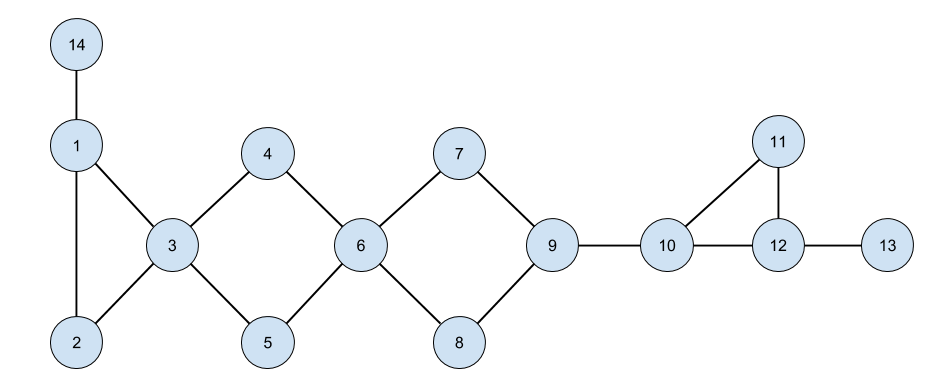
\includegraphics[scale=0.4]{Imagenes/Imagen1}

\noindent
Y bajo esta nueva representación, podemos traducir las consultas de la siguiente forma: \\

\textbf{Tipo A:} dados dos nodos n1 y n2, imprimir la cantidad de puentes en el camino para llegar de n1 a n2.

\textbf{Tipo B:} dado un eje, imprimir un 1 si es un puente, y 0 en caso contrario.

\textbf{Tipo C:} dado un nodo n, imprimir la cantidad de nodos en la componente 2-eje-conexa, menos 1.

\hfill \break \noindent
\textbf{Aclaraciones:}

\underline{Tipo A}: si bien puede existir más de un camino para llegar de un nodo a otro, todos esos camino pasarán por los mismo ejes puentes, si es que existen. Si existieran dos caminos distintos para llegar de un nodo a otro, y cada camino pasase por ejes puentes distintos, entonces no serían puentes.

\underline{Componente 2-eje-conexa}: es una componente que no tiene un puente.

\subsection{Solución}
Dividimos la solución en 3 grandes partes:
\begin{enumerate}
\item Cálculo de puentes
\item Cálculo de componentes 2-eje-conexas
\item Cálculo de puentes en camino
\end{enumerate}

\subsubsection{Cálculo de puentes}
\noindent
Todas las consultas tienen relación algún tipo de relación con ejes puente. Dado que las consultas de tipo B y C deben responderse en tiempo constante, esta información tiene que estar precalculada.
\noindent
Para calcular los ejes puente, utilizamos el algoritmo de \textit{dfs} visto en clase. La única modificación que le hicimos, fue que no guardamos los nodos de articulación.
\noindent
Luego de correr este algoritmo, ya tendremos los ejes puentes distinguidos:

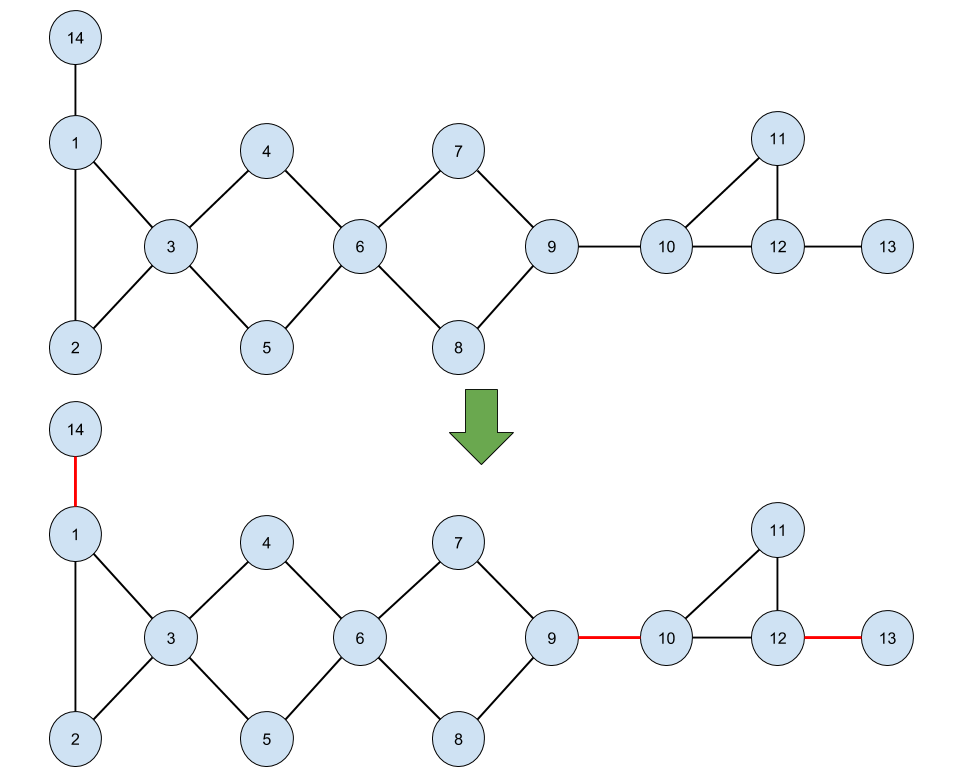
\includegraphics[scale=0.4]{Imagenes/Imagen2}

\subsubsection{Cálculo de componentes 2-eje-conexas}
\noindent
Una vez calculados los puentes, vamos a calcular las componentes 2-eje-conexas. Lo que hacemos es, por cada nodo:
\begin{enumerate}
\item Si está visitado, saltearse los siguientes pasos.
\item Guardar el nodo en una lista.
\item Marcarlo como visitado.
\item Por cada vecino que no esté conectado por un puente, ir al paso 1.
\end{enumerate}

\noindent
Cada vez que ya no pueda visitar más vecinos, en la lista tengo entonces todos los nodos de la componente deseada.

\hfill \break \noindent
Así sería el cálculo de una componente:

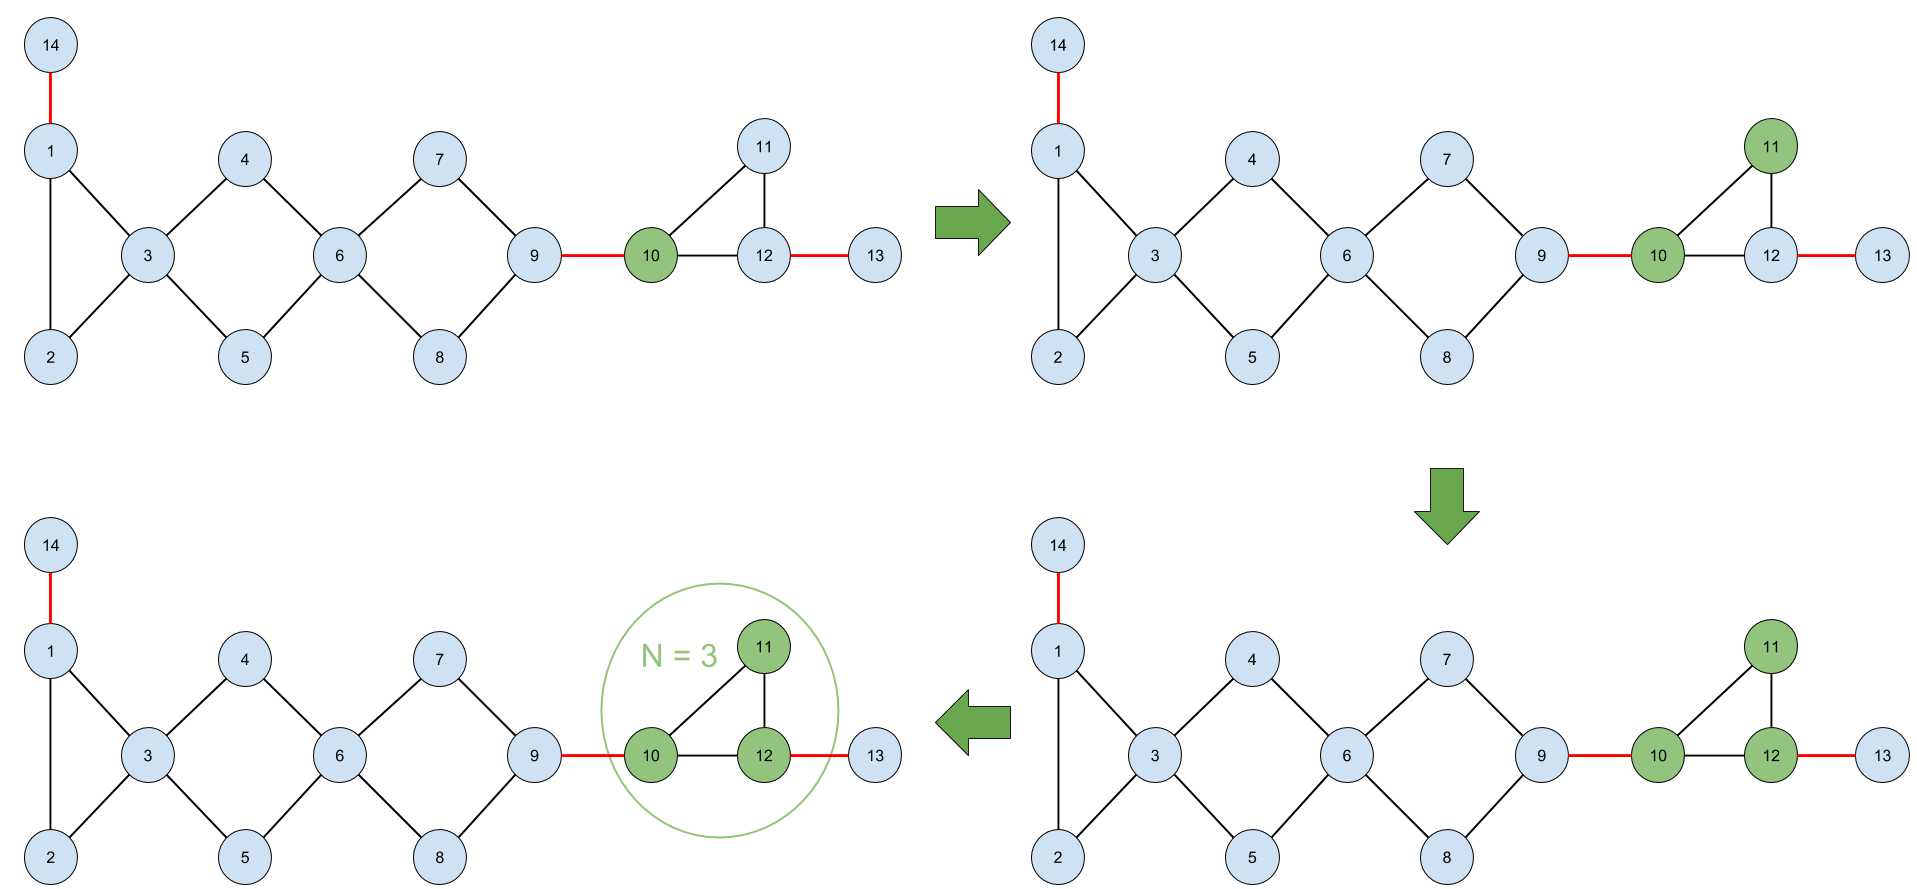
\includegraphics[scale=0.2]{Imagenes/Imagen3}

\hfill \break \noindent
Y así quedaría el grafo luego de calcular todas las componentes:

\hfill \break 
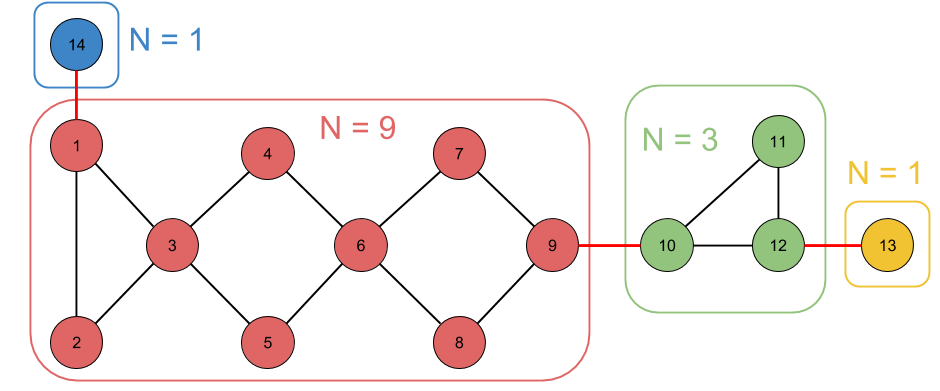
\includegraphics[scale=0.4]{Imagenes/Imagen4}

\noindent
Una vez calculadas todas las distintas componentes, guardamos para cada nodo la cantidad de nodos en la misma componente (menos 1). Esta información nos permitirá responder las consultas de tipo C. 

\subsubsection{Cálculo de puentes en camino}
Para las consultas de tipo A, nos interesa saber la cantidad de puentes en el camino entre dos nodos. Obviamente hablamos de un camino sin nodos repetidos. 

\noindent
En el ejemplo actual, si tenemos la consulta \textit{A 13 14}, un posible camino es el siguiente:

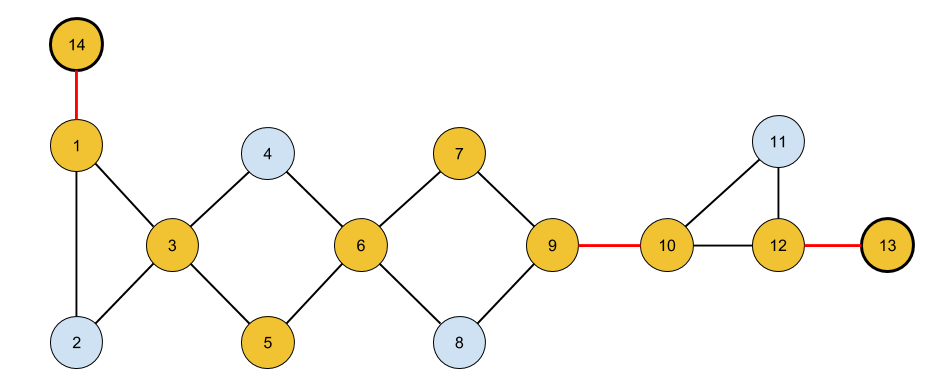
\includegraphics[scale=0.4]{Imagenes/Imagen5}

\hfill \break \noindent
Podemos ver que en camino existen 3 ejes puente, por lo que esa sería la respuesta a la consulta. Ahora, si recibimos esta otra consulta \textit{A 2 8}, un camino posible es el siguiente:

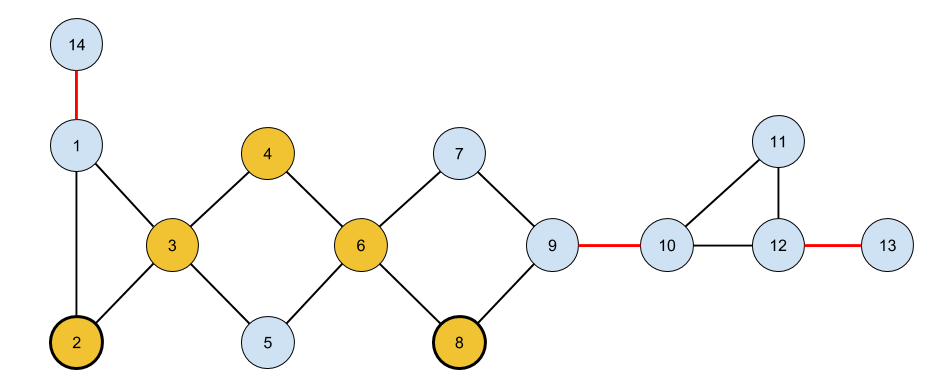
\includegraphics[scale=0.4]{Imagenes/Imagen6}

\noindent
En este caso no cruzamos ningún puente, por lo que la respuesta sería 0. Lo que estamos haciendo entonces es un simple \textit{dfs}, desde uno de los nodos, en busca de otro. Vamos a ir contando los puentes que pasamos en el camino, y sin importar el camino que se tome, la cantidad de puentes va a ser siemple la misma.

\hfill \break \noindent
Una vez resueltos estos tres subproblemas, podremos resolver consultas de tipos A, B y C.

\subsubsection{Complejidad}
\noindent
Nuestro algoritmo tiene las siguientes partes:
\begin{enumerate}
\item Inicialización
\item Cálculo de puentes
\item Cálculo de componentes 2-eje-conexas
\item Resolución de consultas
\begin{enumerate}
\item Tipo A
\item Tipo B
\item Tipo C
\end{enumerate}
\end{enumerate}

\subsubsection{Inicialización}
\noindent
Utilizamos lista de adyacencia para representar el grafo, por lo que la inicialización del mismo tiene complejidad  \O{N + M}. Ahora, como dice la Pista 1, entre todo par de nodos existe un camino, por lo que $N \in$ \O{M}. Entonces, la inicialización termina teniendo costo \O{M}. También inicializamos otras estructuras como vectores de tamaño $N$ y $M$, pero su costo sigue entrando dentro de \O{M}.

\subsubsection{Cálculo de puentes}
\noindent
El algoritmo de cálculo de puentes es el visto en clase. La única modificación hecha fue que no guardamos los nodos de articulación. La implementación es un \textit{dfs} normal, donde cada nodo es visitado una única vez. Su costo es entonces \O{N + M}, pero al igual que en la sección anterior, sabemos que equivale a \O{M}. 

\subsubsection{Cálculo de componentes 2-eje-conexas}
\noindent
Cómo vimos previamente, el algoritmo consiste en correr un \textit{dfs} desde cada nodo, para encontrar todos los nodos dentro de la misma componente. Sin embargo, nos aseguramos de compartir el vector de nodos visitados entre todos los \textit{dfs}. Entonces, en total, cada nodo es visitado una única vez, y cada eje como mucho será recorrido 2 veces. Nos encontramos entonces nuevamente con una complejidad \O{N + M}, que otra vez reemplazamos por \O{M}.

\subsubsection{Resolución de consultas}
\noindent
\textbf{Tipo A}\\
\noindent
Ya leer las consultas de tipo A nos toma \O{Q_A}. Ahora, por cada consulta, queremos poder calcular la cantidad de puentes en el camino. Como dijimos antes, vamos a hacer un \textit{dfs} desde uno de los nodos, en busca del otro. Esto nuevamente (y por última vez) tiene una complejidad una complejidad \O{N + M}. Y otra vez, reemplazamos por \O{M}. Entonces, en total, el costo termina siendo \O{M Q_A}

\hfill \break \noindent
\textbf{Tipo B}\\
\noindent
Las consultas de tipo B se responden en tiempo constante, ya que previamente calculamos los ejes puente. Entonces, terminamos teniendo complejidad \O{Q_B}.

\hfill \break \noindent
\textbf{Tipo C}\\
\noindent
Las consultas de tipo C también se pueden responder en tiempo constante, ya que previamente calculamos para cada nodo la cantidad de nodos en la misma componente 2-eje-conexa. Entonces, responder este tipo de consulta tiene complejidad \O{Q_C}.


\subsubsection{Conclusión}
\noindent
Resumiendo, estas fueron las complejidades calculadas:\\
\textbf{Inicialización:} \O{M}\\
\textbf{Cálculo de puentes:} \O{M}\\
\textbf{Cálculo de componentes 2-eje-conexas:} \O{M}\\
\textbf{\underline{Resolución de consultas}:}\\
\textbf{  Tipo A:} \O{M Q_A}\\
\textbf{  Tipo B:} \O{Q_B}\\
\textbf{  Tipo C:} \O{Q_C}\\

\noindent
Sumando cada una de estas complejidades, terminamos con: \O{M + M Q_A + Q_B + Q_C}

\subsection{Puntaje}
El peso otorgado a este ejercicio es: 9



